% Shared standalone design for the editable figure reconstructions.
\documentclass[tikz,border=5pt,10pt]{standalone}
\usepackage[T1]{fontenc}
\usepackage[utf8]{inputenc}
\usepackage{newpxtext,newpxmath}
\usepackage[scaled=.94]{sourcesanspro}
\usepackage{pgfplots}
\pgfplotsset{compat=1.18}
\usetikzlibrary{arrows.meta,calc,positioning,decorations.pathreplacing,
  decorations.markings,patterns,matrix,shapes.geometric,fit,backgrounds,
  intersections,angles,quotes}
\definecolor{ink}{HTML}{203746}
\definecolor{accent}{HTML}{146C78}
\definecolor{muted}{HTML}{667780}
\definecolor{signalred}{HTML}{B94B44}
\color{ink}
\tikzset{>=Latex,line width=.8pt,
  every node/.style={font=\small},
  axis/.style={->,draw=muted,line width=.5pt},
  guide/.style={draw=muted,dashed,line width=.45pt},
  curve/.style={draw=accent,line width=1pt},
  marker/.style={circle,fill=accent,inner sep=1.5pt},
  labelbox/.style={fill=white,inner sep=2pt}}

\begin{document}
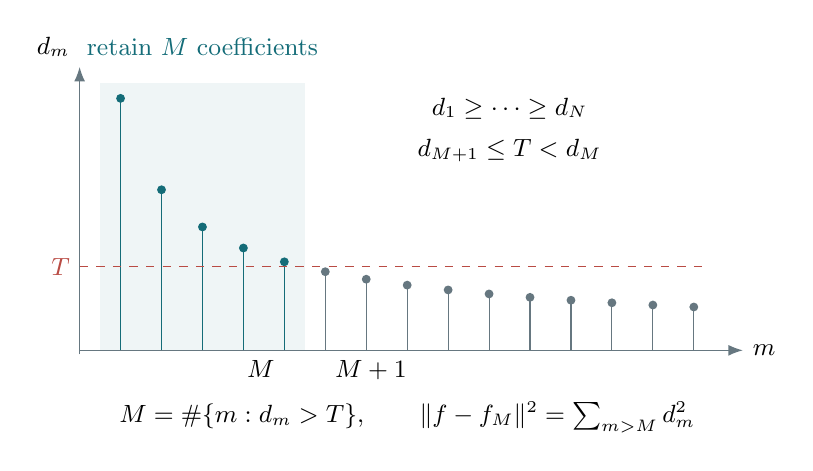
\begin{tikzpicture}[x=.52cm,y=1cm]
\draw[axis] (0,0)--(16.2,0) node[right] {$m$};\draw[axis] (0,-.05)--(0,3.6) node[above left] {$d_m$};
\fill[accent!7] (.5,0) rectangle (5.5,3.4);
\draw[accent] (1,0)--(1,3.20000000);\fill[accent] (1,3.20000000) circle(1.6pt);
\draw[accent] (2,0)--(2,2.03929700);\fill[accent] (2,2.03929700) circle(1.6pt);
\draw[accent] (3,0)--(3,1.56682742);\fill[accent] (3,1.56682742) circle(1.6pt);
\draw[accent] (4,0)--(4,1.29960383);\fill[accent] (4,1.29960383) circle(1.6pt);
\draw[accent] (5,0)--(5,1.12413760);\fill[accent] (5,1.12413760) circle(1.6pt);
\draw[muted] (6,0)--(6,0.99850827);\fill[muted] (6,0.99850827) circle(1.6pt);
\draw[muted] (7,0)--(7,0.90330882);\fill[muted] (7,0.90330882) circle(1.6pt);
\draw[muted] (8,0)--(8,0.82821194);\fill[muted] (8,0.82821194) circle(1.6pt);
\draw[muted] (9,0)--(9,0.76717130);\fill[muted] (9,0.76717130) circle(1.6pt);
\draw[muted] (10,0)--(10,0.71639076);\fill[muted] (10,0.71639076) circle(1.6pt);
\draw[muted] (11,0)--(11,0.67335600);\fill[muted] (11,0.67335600) circle(1.6pt);
\draw[muted] (12,0)--(12,0.63632966);\fill[muted] (12,0.63632966) circle(1.6pt);
\draw[muted] (13,0)--(13,0.60406935);\fill[muted] (13,0.60406935) circle(1.6pt);
\draw[muted] (14,0)--(14,0.57566093);\fill[muted] (14,0.57566093) circle(1.6pt);
\draw[muted] (15,0)--(15,0.55041551);\fill[muted] (15,0.55041551) circle(1.6pt);
\draw[signalred,dashed] (0,1.0613229358560023) node[left] {$T$}--(15.4,1.0613229358560023);
\node[below left] at (5,0) {$M$};\node[below right] at (6,0) {$M+1$};
\node[accent,align=center] at (3,3.85) {retain $M$ coefficients};
\node[align=center] at (10.5,2.8) {$d_1\geq\cdots\geq d_N$\\[4pt]$d_{M+1}\leq T<d_M$};
\node at (8,-.85) {$M=\#\{m:d_m>T\},\qquad \|f-f_M\|^2=\sum_{m>M}d_m^2$};
\end{tikzpicture}
\end{document}
